\section{Perceptron}

Das Perceptron ist eine einfache Variante eines neuronalen Netzes. Das Prinzip wurde erstmals im Jahre 1958 von Frank Rosenblatt veröffentlicht\cite{rosenblatt58}. Es handelt sich dabei um eine lineare Diskriminantenfunktion. Während des Lernvorganges wird ein Vektor mit Gewichten erstellt, welcher dann anschließend eine Klassifikation vornimmt. Das Ergebnis wird anschließend durch eine Signum-Funktion dargstellt.

\subsection{Untersuchen sie den Trainingsalgorithmus: Welche Eigenschaften der Daten beeinflussen die durchschnittliche Anzahl an Iterationen bis eine Lsung w* gefunden wurde?}

\subsection{Welchen Einufluss hat die Schrittweite?}
\subsection{Plotten Sie Daten und Entscheidungsgrenze (analog zu Punkt 1.1).}
\begin{figure}
	
	\centering
	\mbox{
		\subfigure[Nicely spread data]{
			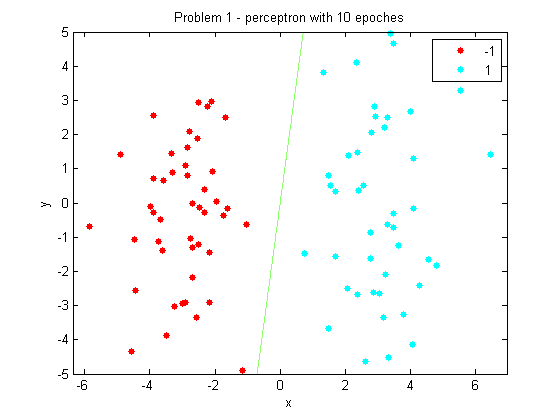
\includegraphics[width=60mm, trim = 0cm 0cm 0cm 0cm]{img/goodsep1.png}
		}
		
		\subfigure[seperable data but close together]{
			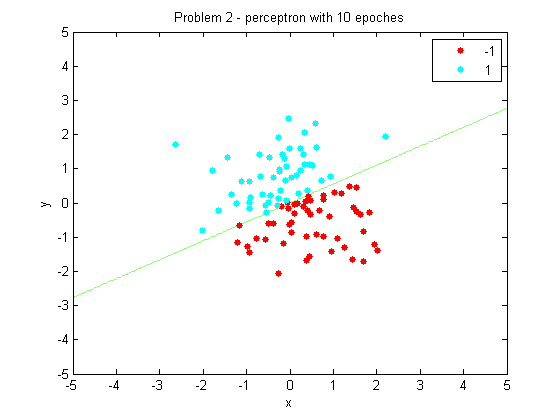
\includegraphics[width=60mm, trim = 0cm 0cm 0cm 0cm]{img/closesep2.png}
		}	
	}
	\mbox{
		\subfigure[Not seperable data]{
			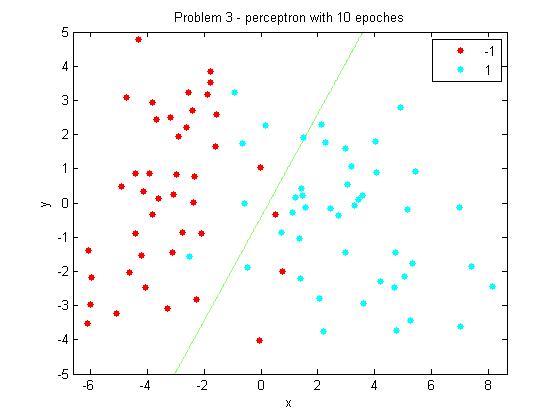
\includegraphics[width=60mm, trim = 0cm 0cm 0cm 0cm]{img/notsep3.png}
		}
	}
	
	\caption{Verschiedene plots der Perceptron Klassifier nach 10 Epochen}
	\label{fig:perceptron}
\end{figure}

\subsection{Vergleichen Sie das Perzeptron mit der Funktion memory. Worin liegt der Unterschied?}
\subsection{Wie ist das Verhalten bei nicht linear separierbaren Daten?}